\documentclass[11pt,a4paper]{article}

\usepackage[utf8]{inputenc}
\usepackage[T1]{fontenc}
\usepackage[a4paper, margin=1in]{geometry}
\usepackage{amsmath, amssymb, amsthm, mathtools}
\usepackage{graphicx}
\usepackage{tikz}
\usetikzlibrary{arrows.meta, decorations.markings, positioning}
\usepackage{booktabs, array}
\usepackage{hyperref}
\usepackage{xcolor}
\usepackage{authblk}
\usepackage{bm}
\usepackage{siunitx}
\usepackage{caption}
\hypersetup{colorlinks=true, linkcolor=blue!60!black, citecolor=green!50!black, urlcolor=blue!60!black}

% ── Physics macros ──────────────────────────────────────────────────────
\newcommand{\N}{\mathcal{N}}
\newcommand{\Tr}{\operatorname{Tr}}
\newcommand{\U}{\mathrm{U}}
\newcommand{\SU}{\mathrm{SU}}
\newcommand{\SO}{\mathrm{SO}}
\newcommand{\Sp}{\mathrm{Sp}}
\newcommand{\USp}{\mathrm{USp}}
\newcommand{\adj}{\mathrm{adj}}
\newcommand{\fund}{\square}
\newcommand{\afund}{\bar{\square}}
\newcommand{\Rch}{R}
\newcommand{\abar}{\bar{a}}
\newcommand{\Bcond}{\mathcal{B}}
\newcommand{\Nf}{N_{\!f}}
\newcommand{\Nc}{N}

% ── Title ──────────────────────────────────────────────────────────────
\title{\bfseries IR fixed points and RG phases of $\SU(N)\times\SU(N)$\\
  quiver gauge theories in the non-Veneziano large-$N$ limit}
\author{%
  % AUTHOR PLACEHOLDER
}
\date{\today}

\begin{document}
\maketitle

\begin{abstract}
\noindent
We classify four-dimensional $\N=1$ asymptotically free
$\SU(N)_{1}\times\SU(N)_{2}$ quiver gauge theories admitting a
non-trivial large-$N$ limit without Veneziano scaling of fundamental
matter, and analyse the superconformal fixed points and
renormalisation-group flow phases that arise in the two-coupling
plane.  Nine universality classes emerge; every class with a
well-defined leading-$N$ $a$-maximum satisfies $a=c$ to leading order
in $1/N$, and each class contains multiple distinct quiver
representatives.  Applying the boundary analysis of
Intriligator--Wecht (\texttt{hep-th/0502049}) to both axis SCFTs, we
compute the boundary one-loop coefficients
$b_{0}^{(a)}(g_{b}^{\star})$ and classify each class by the sign
pattern of their leading-$N$ coefficients, obtaining the flow
topology in the $(g_{1},g_{2})$-plane for every class.  As our main
result, we exhibit an explicit realisation of the
``both axes IR-stable'' topology (Figure~6 of \cite{IW2005}), which
those authors noted they could not construct: deforming class~16 by
$\Nf$ fundamentals on node~2 in the window
$0.427\,N-1<\Nf<N-1$ yields precisely this phase.
\end{abstract}

\tableofcontents
\bigskip
\hrule
\bigskip

% ══════════════════════════════════════════════════════════════════════
\section{Introduction}
\label{sec:intro}

% INTRO PLACEHOLDER
% ══════════════════════════════════════════════════════════════════════
% § 1   Introduction
% ══════════════════════════════════════════════════════════════════════

Four-dimensional $\N=1$ gauge theories with multiple gauge group factors
often flow in the infra-red to superconformal field theories with a
continuous family of exactly marginal couplings, parameterised by the
independent ratios of the gauge couplings of the individual factors.  In
two-coupling systems one may then ask how the RG flow in the
$(g_{0},g_{1})$ plane organises itself between the Gaussian fixed point
in the ultra-violet and the available infra-red fixed points --- both the
interacting interior fixed point (when it exists) and the
``boundary'' fixed points associated with decoupling one of the two
gauge groups.

A systematic answer at large $N$ was given by Intriligator and
Wecht~\cite{IW2005}: at each boundary one $a$-maximises the decoupled
sub-quiver to obtain R-charges, and asks whether the second gauge
coupling is relevant or irrelevant at that fixed point.  This criterion
is encoded in the anomalous-dimension combination
\begin{equation}
  \Bcond_{a}\;=\;\Tr\!\bigl[R^{(a)}\,G_{a}^{2}\bigr]
  \label{eq:Bcond-def-intro}
\end{equation}
computed at the opposite boundary's $a$-max point, whose sign
determines whether the axis is IR-unstable (and hence releases the flow
into the interior) or IR-stable (and hence traps it).  The authors of
\cite{IW2005} identified two representative topologies, reproduced as
Figures~5 and 6 of that paper, corresponding respectively to both
boundaries being IR-unstable (and the flow ending at an interior SCFT
$C$) and both boundaries being IR-stable (so that generic flows are
captured by the single-node axis fixed points).  The latter topology
would require a separatrix between two basins of attraction, and
\cite{IW2005} remarked that they did not find examples of it.

\medskip
In the present paper we close this gap with a systematic scan.  We
classify \emph{all} four-dimensional $\N=1$ asymptotically free
$\SU(N)\times\SU(N)$ quiver gauge theories with only bifundamental
inter-node matter and adjoint/rank-two tensor intra-node matter,
admitting a large-$N$ limit \emph{without} Veneziano scaling of
fundamental matter (i.e.\ with no fundamentals whose number grows
linearly with $N$).  Seven universality classes emerge, each having
$a=c$ to leading order in $1/N$ and each falling into one of three RG
phases depending on the sign pattern of its two boundary functions
$(\Bcond_{A},\Bcond_{B})$:

\begin{itemize}
  \item Both IR-unstable --- interior SCFT $C$ is the global IR
        attractor.  This is the phase of \cite[Fig.~5]{IW2005}.
  \item Mixed --- one axis attracts, the other repels.  Generic flows
        end on the attracting axis SCFT; $C$ is either a saddle or a
        non-global attractor.
  \item Both IR-stable --- the axes trap every generic flow.  This is
        the phase of \cite[Fig.~6]{IW2005}, which had not previously
        been explicitly realised.
\end{itemize}

Our main result is that the last phase is accessible within the
classified database by a single-parameter deformation:
deforming the eight-theory class~16 (with matter content
$A+2\bar A$ on node~$0$, $\bar A$ on node~$1$, and three bifundamentals)
by adding $\Nf$ fundamentals on node~$1$ in the window
\begin{equation}
  0.427\,N-1\;<\;\Nf\;<\;N-1\,,
  \label{eq:main-window}
\end{equation}
we find $b_{0}^{(0,1)}>0$ (both nodes UV-asymptotically free) while
$\Bcond_{A}$ and $\Bcond_{B}$ are \emph{both} negative, i.e.\ both axis
fixed points are IR-stable, in precise correspondence with
\cite[Fig.~6]{IW2005}.

\medskip
The rest of the paper is organised as follows.  Section~\ref{sec:setup}
fixes conventions and spells out the large-$N$ and non-Veneziano limits.
Section~\ref{sec:classification} describes the enumeration and
$a$-maximisation pipeline and reports the seven equal-rank universality
classes.  Section~\ref{sec:boundary} reviews the boundary prescription
\cite{IW2005} and tabulates the corrected asymptotic-freedom budget
$\Bcond$ for each class.  Section~\ref{sec:phases} classifies each
class's RG flow topology and presents the Figure~6 realisation.
Section~\ref{sec:discussion} discusses implications and open
directions; Appendix~\ref{app:mixed} collects the mixed-rank
$\SU(m_{0}N)\times\SU(m_{1}N)$ data.


% ══════════════════════════════════════════════════════════════════════
\section{Setup: two-node quivers in the non-Veneziano large-$N$ limit}
\label{sec:setup}

% ══════════════════════════════════════════════════════════════════════
% § 2   Setup
% ══════════════════════════════════════════════════════════════════════

\subsection{Field content and gauge group}
\label{sec:setup-content}

We consider four-dimensional $\N=1$ gauge theories whose gauge group is
\begin{equation}
  G\;=\;\SU(N)_{1}\times\SU(N)_{2},
  \label{eq:gauge-group}
\end{equation}
with a common rank parameter $N$ that will be taken to infinity.  The
allowed chiral matter is organised into \emph{node matter}, transforming
only under one of the two factors, and \emph{inter-node matter},
bifundamentals charged under both factors.

At node $a\in\{1,2\}$ we allow the adjoint and the rank-two tensors of
$\SU(N)$,
\begin{equation}
  \{\adj,\;S,\;\bar S,\;A,\;\bar A\}\,,
  \label{eq:node-matter}
\end{equation}
with the representation-theoretic data collected in
Table~\ref{tab:SU-reps}.  We denote the multiplicities by
$(n_{\adj}^{(a)},n_{S}^{(a)},n_{\bar S}^{(a)},n_{A}^{(a)},n_{\bar A}^{(a)})$.

\begin{table}[h]
  \centering
  \begin{tabular}{lccc}
    \toprule
    Representation & Dimension & $T(r)$ & Anomaly $\mathcal A(r)$ \\
    \midrule
    $\fund$ & $N$            & $1/2$       & $+1$ \\
    $\afund$& $N$            & $1/2$       & $-1$ \\
    $\adj$  & $N^{2}-1$      & $N$         & $0$  \\
    $S$     & $N(N{+}1)/2$   & $(N{+}2)/2$ & $+(N{+}4)$ \\
    $\bar S$& $N(N{+}1)/2$   & $(N{+}2)/2$ & $-(N{+}4)$ \\
    $A$     & $N(N{-}1)/2$   & $(N{-}2)/2$ & $+(N{-}4)$ \\
    $\bar A$& $N(N{-}1)/2$   & $(N{-}2)/2$ & $-(N{-}4)$ \\
    \bottomrule
  \end{tabular}
  \caption{Dynkin indices and cubic anomalies of the $\SU(N)$
    representations used, with $T(\square)\equiv 1/2$.}
  \label{tab:SU-reps}
\end{table}

Between the two nodes we admit bifundamental chiral multiplets with
either orientation,
\begin{equation}
  (\fund_{1},\afund_{2})^{k_{+-}},
  \quad
  (\afund_{1},\fund_{2})^{k_{-+}},
  \quad
  (\fund_{1},\fund_{2})^{k_{++}},
  \quad
  (\afund_{1},\afund_{2})^{k_{--}}\,.
\end{equation}
Higher $\SU(N)_{1}\times\SU(N)_{2}$ representations
(e.g.\ $(\fund,\adj)$) are excluded: any inter-node field whose
representation dimension grows as $\sim N^{2}$ on either factor would
contribute $\sim N^{2}$ to the one-loop matter sum
$\sum_{i}T_{G_{a}}(r_{a,i})\dim(r_{b,i})$ and immediately destroy
asymptotic freedom in the large-$N$ limit.

Finally, we may add $\Nf^{(a)}$ vector-like pairs of (anti-)fundamentals
on node $a$, $(\fund+\afund)^{\Nf^{(a)}}$.  In the \emph{non-Veneziano}
limit defined below $\Nf^{(a)}$ is of order $N^{0}$.

\subsection{Anomaly cancellation and the one-loop beta function}
\label{sec:setup-beta}

Absence of the $\SU(N)^{3}_{a}$ cubic gauge anomaly at node $a$ is a
\emph{gauge-invariance requirement that must hold identically in
$N$}: it is a polynomial equation in $N$ whose $N^{1}$ and $N^{0}$
coefficients must vanish \emph{separately and exactly}.  The full
anomaly equation at node $a$ reads
\begin{equation}
  N\,(\deg^{+}_{a}-\deg^{-}_{a})
  +\bigl(n_{S}^{(a)}-n_{\bar S}^{(a)}\bigr)(N+4)
  +\bigl(n_{A}^{(a)}-n_{\bar A}^{(a)}\bigr)(N-4)
  +\bigl(\Nf^{(a),+}-\Nf^{(a),-}\bigr)\;\equiv\;0\,,
  \label{eq:anomaly}
\end{equation}
where $\deg^{\pm}_{a}$ counts outgoing/incoming bifundamentals at
node $a$.  The identity~\eqref{eq:anomaly} in $N$ is equivalent to
the two independent conditions
\begin{align}
  \text{$N$-coefficient:} \quad
  &\bigl(\deg^{+}_{a}-\deg^{-}_{a}\bigr)
   +\bigl(n_{S}^{(a)}-n_{\bar S}^{(a)}\bigr)
   +\bigl(n_{A}^{(a)}-n_{\bar A}^{(a)}\bigr)\;=\;0\,,
   \label{eq:anomaly-N}\\[2pt]
  \text{constant:} \quad
  &4\bigl(n_{S}^{(a)}-n_{\bar S}^{(a)}\bigr)
   -4\bigl(n_{A}^{(a)}-n_{\bar A}^{(a)}\bigr)
   +\bigl(\Nf^{(a),+}-\Nf^{(a),-}\bigr)\;=\;0\,,
   \label{eq:anomaly-const}
\end{align}
both of which are imposed exactly.  In particular, the chiral excess
of fundamentals $\Nf^{(a),+}-\Nf^{(a),-}$ is fixed by
\eqref{eq:anomaly-const} once the tensor multiplicities are chosen,
and may be non-zero even when $\Nf^{(a),+}+\Nf^{(a),-}$ is
$\mathcal O(N^{0})$ (see Section~\ref{sec:setup-largeN} below).

The one-loop coefficient in
$\beta(g_{a})=-\,g_{a}^{3}\,b_{0}^{(a)}/(16\pi^{2})+\mathcal O(g_{a}^{5})$ is
\begin{equation}
  b_{0}^{(a)}\;=\;3\,T(\adj_{a})\;-\;\sum_{i\in\text{matter}}T_{G_{a}}(r_{i})\,,
  \label{eq:b0}
\end{equation}
and for the matter content above
\begin{equation}
  b_{0}^{(a)}\;=\;3N\;-\;n_{\adj}^{(a)}N
  -\tfrac{N+2}{2}(n_{S}^{(a)}+n_{\bar S}^{(a)})
  -\tfrac{N-2}{2}(n_{A}^{(a)}+n_{\bar A}^{(a)})
  -\tfrac{k_{\text{tot}}}{2}\,N
  -\tfrac{1}{2}\Nf^{(a)}\,,
  \label{eq:b0-SU}
\end{equation}
where
$k_{\text{tot}}\equiv k_{++}+k_{--}+k_{+-}+k_{-+}$ is the total number
of bifundamental fields (identical at the two nodes by bifundamental
symmetry) and $\Nf^{(a)}\equiv\Nf^{(a),+}+\Nf^{(a),-}$.

\subsection{The non-Veneziano large-$N$ limit and the bound $k_{\text{tot}}\le 4$}
\label{sec:setup-largeN}

Writing \eqref{eq:b0-SU} as
$b_{0}^{(a)}(N)=\alpha^{(a)}\,N+\gamma^{(a)}$, asymptotic freedom at
large $N$ requires $\alpha^{(a)}\ge 0$ for both nodes.  The
\emph{Veneziano limit} admits $\Nf^{(a)}\sim N$ and thereby devotes an
$\mathcal O(N)$ portion of the AF budget to fundamentals; we define the
complementary limit.

\begin{quote}
  \textbf{Non-Veneziano limit.}  A two-node quiver is
  \emph{non-Veneziano} if $\Nf^{(a)}=\mathcal O(N^{0})$ at both nodes.
  Equivalently, the AF budget $\alpha^{(a)}$ is absorbed entirely by
  adjoints, rank-two tensors and bifundamentals in \eqref{eq:b0-SU},
  with no $\mathcal O(N)$ contribution from fundamentals.
\end{quote}

The non-Veneziano condition, combined with the \emph{exact}
anomaly-cancellation identity~\eqref{eq:anomaly}, imposes a
non-trivial constraint on the tensor and bifundamental content of
each node: the chiral excess
$\Nf^{(a),+}-\Nf^{(a),-}$ is $\mathcal O(N^{0})$ and hence cannot
absorb any $\mathcal O(N)$ imbalance in~\eqref{eq:anomaly-N}.  In
consequence, \eqref{eq:anomaly-N} must hold \emph{from the tensor
and bifundamental content alone}:
\begin{equation}
  \bigl(\deg^{+}_{a}-\deg^{-}_{a}\bigr)
   +\bigl(n_{S}^{(a)}-n_{\bar S}^{(a)}\bigr)
   +\bigl(n_{A}^{(a)}-n_{\bar A}^{(a)}\bigr)\;=\;0\,,
  \qquad a=1,2,\ \text{(non-Veneziano).}
  \label{eq:anomaly-N-nonVen}
\end{equation}
The constant condition~\eqref{eq:anomaly-const} is then absorbed by
a finite, $\mathcal O(N^{0})$ chiral excess of fundamentals.

At leading order in $1/N$, the AF conditions become
\begin{equation}
  3\;-\;n_{\adj}^{(a)}\;-\;\tfrac{1}{2}\bigl(n_{S}^{(a)}+n_{\bar S}^{(a)}
  +n_{A}^{(a)}+n_{\bar A}^{(a)}\bigr)\;-\;\tfrac{k_{\text{tot}}}{2}
  \;\ge\;0\,,\qquad a=1,2\,.
  \label{eq:AF-lead}
\end{equation}

\paragraph{Why $k_{\text{tot}}\le 4$.}
The leading-$N$ bound \eqref{eq:AF-lead} with
$n_{\adj}^{(a)}=n_{S}^{(a)}=n_{\bar S}^{(a)}=n_{A}^{(a)}=n_{\bar A}^{(a)}=0$
forces
\begin{equation}
  k_{\text{tot}}\;\le\;6\,,
  \label{eq:k-strict}
\end{equation}
saturating at $k_{\text{tot}}=6$ only with no node matter at all, which
yields the trivial class in which both nodes are at the strict
boundary of asymptotic freedom and no rank-two tensor or adjoint may
be added.  In the physically interesting enumeration we require
$b_{0}^{(a)}>0$ \emph{strictly} at leading $N$ in order to have a
non-degenerate RG flow and to admit \emph{some} rank-two tensor or
adjoint matter at either node (otherwise the two nodes are decoupled
pure Yang--Mills with bifundamental matter only, and the universality
class contains no internal structure).  The bound \eqref{eq:AF-lead}
then becomes
\begin{equation}
  k_{\text{tot}}\;\le\;5\,;
\end{equation}
and for the classification presented here we impose the slightly
stronger pragmatic cap
\begin{equation}
  k_{\text{tot}}\;\le\;4\,,
\end{equation}
under which every equal-rank non-Veneziano universality class admits at
least one representative with \emph{both} $n_{\text{tensors}}^{(a)}\ge
1$ and $\Nf^{(a)}=0$.  We have verified by enumeration that the
$k_{\text{tot}}=5$ sector contains no additional equal-rank
non-Veneziano universality classes beyond those captured at
$k_{\text{tot}}\le 4$: the strict saturation
$b_{0}^{(a)}\big|_{\text{leading}}=0$ forces all matter to be
subleading, producing only further instances of the marginal class
already present at $k_{\text{tot}}=4$ (class 44 below).

\subsection{IR fixed points and \texorpdfstring{$a$}{a}-maximisation}
\label{sec:setup-amax}

At a non-trivial IR fixed point the superconformal $R$-symmetry
$R^{\star}$ is the unique non-anomalous combination that maximises
the trial $a$-function~\cite{IntriligatorWecht2003}
\begin{equation}
  a(R)\;=\;\tfrac{3}{32}\,\bigl(3\,\Tr R^{3}-\Tr R\bigr)\,,
  \label{eq:a-trial}
\end{equation}
subject to the gauge-anomaly-free condition at each node $a$,
\begin{equation}
  T(\adj_{a})\;+\;\sum_{i}T_{G_{a}}(r_{i})\,\bigl(R[\Phi_{i}]-1\bigr)\;=\;0\,.
  \label{eq:anomaly-free}
\end{equation}
We retain only the leading $N^{2}$ terms in $a$ and $c$ throughout.

\subsection{Axis SCFTs and the boundary one-loop coefficient
  \texorpdfstring{$b_{0}^{(a)}(g_{b}^{\star})$}{b0(a)(gb*)}}
\label{sec:setup-boundary}

The two-coupling theory possesses, in addition to the Gaussian point
$(g_{1},g_{2})=(0,0)$, two \emph{axis SCFTs} at the decoupling limits
$g_{b}\to 0$ (with $b\ne a$).  On the $g_{a}$-axis, node $b$ decouples
and node $a$ runs on its own into a single-node IR fixed point
$g_{a}=g_{a}^{\star}$, obtained by $a$-maximising the sub-theory in
which node $b$ is switched off and the bifundamentals act as
$\Nf^{(a)}$-type flavours of $\SU(N)_{a}$.  Denote the bifundamental
R-charge obtained by this boundary $a$-maximisation by
$R_{\text{bif}}^{(a\star)}$.

The stability of an axis SCFT against turning on the orthogonal
coupling is controlled by the effective one-loop coefficient of the
decoupled node $b$ at the axis-$a$ fixed point.  Linearising
$\beta(g_{b})$ near $g_{b}=0$ with the bifundamentals carrying their
axis-$a$ anomalous dimension
$\gamma_{\text{bif}}^{(a\star)}=3R_{\text{bif}}^{(a\star)}-2$, the NSVZ
denominator gives
\begin{equation}
  \beta(g_{b})\Big|_{g_{b}=0^{+}}\;\propto\;-\,b_{0}^{(b)}(g_{a}^{\star})\,,
\end{equation}
with
\begin{equation}
  \boxed{\;
  b_{0}^{(b)}(g_{a}^{\star})\;=\;T(\adj_{b})\;+\;\sum_{i\text{ at node }b}
    T_{G_{b}}(r_{i})\,\bigl(R_{i}^{(a\star)}-1\bigr)\;}
  \label{eq:b0-boundary}
\end{equation}
where the sum runs over all matter charged under node $b$, with
$R_{i}^{(a\star)}=R_{\text{bif}}^{(a\star)}$ for bifundamentals and
$R_{i}=2/3$ for fields exclusively at node $b$ (which remain free
spectators on the $a$-axis).  The sign of $b_{0}^{(b)}(g_{a}^{\star})$
determines whether the axis $a$ SCFT is
IR-unstable ($>0$) or IR-stable ($<0$) with respect to $g_{b}$.

We emphasise that $b_{0}^{(b)}(g_{a}^{\star})$ is the natural
generalisation of the Gaussian-point coefficient $b_{0}^{(b)}$:
the UV AF inequality $b_{0}^{(b)}>0$ is the statement that the
$b$-direction is relevant at $(g_{1},g_{2})=(0,0)$, and
$b_{0}^{(b)}(g_{a}^{\star})>0$ is the same statement translated to
the axis-$a$ fixed point.  Both are leading-$N$ quantities of the form
$\alpha_{b}^{\star} N + \gamma_{b}^{\star}$.

\paragraph{Sign convention.}  In our conventions, the NSVZ
numerator is $\propto \Tr[R^{\star} G_{b}^{2}]\propto b_{0}^{(b)}$
(with $b_{0}^{(b)}>0$ meaning the gauge coupling is relevant, as in the
UV).  Thus ``$b_{0}^{(b)}(g_{a}^{\star})>0$, axis $a$ is IR-unstable,
flow released into the interior'' — matching our convention that
asymptotic freedom corresponds to $b_{0}>0$.

\subsection{Database and scope}
\label{sec:setup-scope}

All numerical data used throughout this paper come from a symbolic
large-$N$ $a$-maximisation pipeline, producing a database of $4{,}560$
two-node theories grouped into $135$ universality classes by their
$a$-maxima.  We focus on the $\SU(N)\times\SU(N)$ equal-rank sector in
the non-Veneziano limit, where \emph{seven} universality classes arise
(Section~\ref{sec:classification}); their boundary coefficients
$b_{0}^{(a)}(g_{b}^{\star})$ are tabulated in
Section~\ref{sec:boundary}, and the resulting RG-flow topology of each
class is given in Section~\ref{sec:phases}.


% ══════════════════════════════════════════════════════════════════════
\section{Classification via \texorpdfstring{$a$}{a}-maximisation}
\label{sec:classification}

% ══════════════════════════════════════════════════════════════════════
% § 3   Classification
% ══════════════════════════════════════════════════════════════════════

\subsection{Enumeration pipeline}
\label{sec:class-enumeration}

We enumerate the equal-rank non-Veneziano sector as follows.  Fix the
bifundamental multiplicity vector
$k=(k_{++},k_{--},k_{+-},k_{-+})$ with total
$k_{\text{tot}}\le 4$ (cf.~Section~\ref{sec:setup-largeN}) and, for
each such $k$, scan the allowed tensor multiplicity tuples
$(n_{\adj}^{(a)},n_{S}^{(a)},n_{\bar S}^{(a)},n_{A}^{(a)},n_{\bar A}^{(a)})$
at each node subject to:
\begin{enumerate}\setlength{\itemsep}{2pt}
  \item the leading-$N$ asymptotic-freedom condition
    \eqref{eq:AF-lead} at each node;
  \item the cubic-anomaly cancellation \eqref{eq:anomaly}
    \emph{exactly} (i.e.\ identically in $N$), enforced as the two
    separate equations \eqref{eq:anomaly-N}
    and~\eqref{eq:anomaly-const}.  In the non-Veneziano sector
    \eqref{eq:anomaly-N-nonVen} fixes an integer linear relation
    between the bifundamental chiral excess and the tensor
    multiplicities at each node, and the remaining
    $\mathcal O(N^{0})$ discrepancy in~\eqref{eq:anomaly-const} is
    absorbed by a finite chiral excess of fundamentals
    $\Nf^{(a),+}-\Nf^{(a),-}\in\mathbb Z$;
  \item discrete symmetries exchanging the two nodes, reflecting
    bifundamentals $(\fund\leftrightarrow\afund)$ at each end
    independently, and orienting the bifundamental edges.
\end{enumerate}
The enumeration is implemented in \texttt{quiver\_generation.py}, in
which the function \texttt{chiral\_excess\_coeffs(\ldots)} returns
the coefficients $(a_{N},a_{0})$ such that the required chiral
excess is $\Nf^{(a),+}-\Nf^{(a),-}=a_{N}\,N+a_{0}$; in the
non-Veneziano sector the scan is restricted to quivers with
$a_{N}=0$, so the excess is $\mathcal O(N^{0})$ as demanded by the
non-Veneziano definition.
Each surviving theory is then subjected to symbolic
$a$-maximisation: the R-charge manifold is parameterised by
\eqref{eq:anomaly-free}, $a(R)$ of \eqref{eq:a-trial} is extremised
symbolically, and only critical points inside the allowed polytope
with negative-definite Hessian are retained.  Theories sharing the
same value of $a/N^{2}$ (to $10^{-10}$ numerical precision after
algebraic simplification) are grouped into a universality
class.\footnote{We use the class labels of the global $135$-class
table of the full database without relabelling.}  A universality class
may contain theories with genuinely distinct matter and/or edge
structure, as illustrated below.

\paragraph{Flat-direction (nonSCFT) theories.}
A small number of quivers admit a \emph{flat direction} at the
critical point of the $a$-trial: the Hessian has a zero eigenvalue,
so the critical point is not a genuine local maximum and the IR
R-charges are not uniquely determined.  These theories correspond to
moduli spaces of near-IR R-symmetries rather than to isolated SCFT
fixed points, and the leading-$N$ value of $a$ along the flat
direction is not a well-defined invariant of the class.  Concretely,
20 non-Veneziano theories in the enumeration exhibit such a flat
direction at leading~$N$ — all of them are empty-node quivers in
which one gauge node carries only bifundamental matter and the other
carries a pair of distinct rank-2 tensors with equal multiplicity
(e.g.\ $S+\bar S$ or $A+\bar A$); the leading-$N$ anomaly-free
conditions then conspire to pin $R_{\text{tensor}_1}+R_{\text{tensor}_2}=2$,
making the $a$-trial independent of the difference
$R_{\text{tensor}_1}-R_{\text{tensor}_2}$.  These 20 theories are
assigned to the \emph{nonSCFT} umbrella introduced below (together
with classes~$1$, $9$, and~$877$, all of which likewise fail to
describe a unitary interacting SCFT at leading~$N$) and are excluded
from the nine-class tabulation; the remaining $432-20=412$
non-Veneziano theories distribute among the nine classes summarised
in Table~\ref{tab:nine-classes}.

\subsection{The nine non-Veneziano equal-rank classes}
\label{sec:class-nine}

Nine universality classes satisfy the enumeration constraints above.
Their $a$-charges and representative counts are collected in
Table~\ref{tab:nine-classes}.

\begin{table}[h]
  \centering
  \small
  \setlength{\tabcolsep}{6pt}
  \begin{tabular}{clr}
    \toprule
    Class & $a/N^{2}$ & $\#$\,theories \\
    \midrule
    $1$   & $0$                                             & $6$   \\
    $2$   & $-\tfrac{297}{32}+\tfrac{135\sqrt 5}{32}$          & $32$  \\
    $4$   & $-\tfrac{229}{32}+\tfrac{65\sqrt{13}}{32}$         & $12$  \\
    $9$   & $\tfrac{27}{64}$                                   & $139$ \\
    $16$  & $\tfrac{3}{32}+\tfrac{5\sqrt 5}{32}$               & $8$   \\
    $21$  & $-\tfrac{7}{2}+\tfrac{5\sqrt{10}}{4}$              & $77$  \\
    $23$  & $\tfrac{30159}{86528}+\tfrac{2295\sqrt{17}}{86528}$& $48$  \\
    $44$  & $\tfrac{1}{2}$                                  & $81$  \\
    $877$ & $0$                                             & $9$   \\
    \bottomrule
  \end{tabular}
  \caption{The nine non-Veneziano $\SU(N)\times\SU(N)$ universality
    classes.  $a/N^{2}$ is the exact leading-$N$ central charge;
    $\#$\,theories is the number of distinct non-Veneziano quivers the
    enumeration finds in the class after excluding those with an
    $a$-trial flat direction at leading~$N$ (see text).  All nine
    classes satisfy the leading-$N$ $a=c$ relation.  Classes~$1$,
    $9$, and $877$ are collected in the \emph{nonSCFT umbrella} of
    Section~\ref{sec:class-special} (together with 20 flat-direction
    theories not listed here) because their leading-$N$
    $a$-maximisation does not identify a unitary interacting SCFT;
    class~$877$ specifically collects empty-node representatives with
    a unique leading-$N$ $a$-maximum at $a/N^{2}=0$.}
  \label{tab:nine-classes}
\end{table}

\paragraph{Remark on $a=c$.}
Every class in Table~\ref{tab:nine-classes} with a defined leading-$N$
central charge satisfies $a/c=1$ at leading order in $1/N$ (i.e.\
$\Tr R^{\star}=\Tr R^{\star 3}$ modulo $\mathcal O(N^{0})$ terms).
This is a direct consequence of the absence of Veneziano fundamentals:
it is the $\mathcal O(N)$-many fundamentals that would contribute the
asymmetric term breaking $a=c$ at leading $N$.

\subsection{Multiple representatives per class}
\label{sec:class-representatives}

To demonstrate that each class contains genuinely distinct quivers
--- not just the same theory under trivial relabellings --- we list
in Table~\ref{tab:class-reps} several concrete representatives for
each class with their matter and bifundamental edge structures.
Each row is a separate entry of the database with the same
$a/N^{2}$.  Notation $(i\to j,\epsilon_{i}\epsilon_{j})$ denotes a
bifundamental with orientation from node $i$ to node $j$ and $\pm$
signs on each end indicating fundamental~$(+)$ vs
anti-fundamental~$(-)$; a prefactor denotes multiplicity.

\begin{table}[h]
  \centering
  \small
  \setlength{\tabcolsep}{4pt}
  \begin{tabular}{cllll}
    \toprule
    Class & Node 1 matter & Node 2 matter & Bifundamental edges \\
    \midrule
    $1$  & $\bar A$                    & $\bar A$                  & $(1\!\to\!2,++)$ \\
         & $\bar A$                    & $\bar S$                  & $(1\!\to\!2,++)$ \\
         & $\bar A$                    & $A$                       & $(1\!\to\!2,+-)$ \\
    \midrule
    $2$  & $\bar A$                    & $S+2\bar A$               & $(1\!\to\!2,++)$ \\
         & $A+2\bar A$                 & $\bar A$                  & $(1\!\to\!2,++)$ \\
         & $\bar S + A+\bar A$         & $\bar A$                  & $(1\!\to\!2,++)$ \\
         & $\bar S$                    & $\adj+\bar S$             & $(1\!\to\!2,++)$ \\
         & $\bar A$                    & $\adj+A$                  & $(1\!\to\!2,+-)$ \\
    \midrule
    $4$  & $2A+3\bar A$                & $\bar A$                  & $(1\!\to\!2,++)$ \\
         & $\bar S+2A+2\bar A$         & $\bar A$                  & $(1\!\to\!2,++)$ \\
         & $\adj+A+2\bar A$            & $\bar S$                  & $(1\!\to\!2,++)$ \\
         & $2A+3\bar A$                & $S$                       & $(1\!\to\!2,+-)$ \\
    \midrule
    $9$  & $A+2\bar A$                 & $A+2\bar A$               & $(1\!\to\!2,++)$ \\
         & $A+2\bar A$                 & $S+2\bar A$               & $(1\!\to\!2,++)$ \\
         & $A+2\bar A$                 & $\adj+\bar A$             & $(1\!\to\!2,++)$ \\
         & $\bar S+A+\bar A$           & $\bar S+A+\bar A$         & $(1\!\to\!2,++)$ \\
    \midrule
    $16$ & $A+2\bar A$                 & $\bar A$                  & $2\!\times\!(1\!\to\!2,++),(1\!\to\!2,--)$ \\
         & $A+2\bar A$                 & $A$                       & $(1\!\to\!2,++),(1\!\to\!2,+-),(1\!\to\!2,--)$ \\
         & $A+2\bar A$                 & $\bar A$                  & $(1\!\to\!2,++),(1\!\to\!2,+-),(2\!\to\!1,+-)$ \\
         & $A+2\bar A$                 & $A$                       & $2\!\times\!(1\!\to\!2,+-),(2\!\to\!1,+-)$ \\
    \midrule
    $21$ & $A+\bar A$                  & $2\adj$                   & $(1\!\to\!2,++),(1\!\to\!2,--)$ \\
         & $\adj$                      & $2\adj$                   & $(1\!\to\!2,++),(1\!\to\!2,--)$ \\
         & $A+3\bar A$                 & $2\bar A$                 & $2\!\times\!(1\!\to\!2,++)$ \\
         & $2\bar A$                   & $2A+2\bar A$              & $(1\!\to\!2,++),(1\!\to\!2,+-)$ \\
         & $S+\bar S+A+\bar A$         & $\adj$                    & $(1\!\to\!2,++),(1\!\to\!2,--)$ \\
    \midrule
    $23$ & $A+2\bar A$                 & $2A+3\bar A$              & $(1\!\to\!2,++)$ \\
         & $A+2\bar A$                 & $\adj+A+2\bar A$          & $(1\!\to\!2,++)$ \\
         & $2A+3\bar A$                & $\adj+\bar S$             & $(1\!\to\!2,++)$ \\
         & $A+2\bar A$                 & $3A+2\bar A$              & $(1\!\to\!2,+-)$ \\
    \midrule
    $44$ & $2A+3\bar A$                & $2A+3\bar A$              & $(1\!\to\!2,++)$ \\
         & $\adj+A+2\bar A$            & $\adj+A+2\bar A$          & $(1\!\to\!2,++)$ \\
         & $2\adj$                     & $2\adj$                   & $(1\!\to\!2,++),(1\!\to\!2,--)$ \\
         & $A+\bar A$                  & $\adj$                    & $2\!\times\!(1\!\to\!2,++),2\!\times\!(1\!\to\!2,--)$ \\
         & ---                         & ---                       & $3\!\times\!(1\!\to\!2,++),3\!\times\!(1\!\to\!2,--)$ \\
    \midrule
    $877$& ---                         & $A+\bar A$                & $(1\!\to\!2,++),(1\!\to\!2,--)$ \\
         & ---                         & $2A+2\bar A$              & $(1\!\to\!2,++),(1\!\to\!2,--)$ \\
         & $A+3\bar A$                 & ---                       & $(1\!\to\!2,++),(1\!\to\!2,+-)$ \\
         & $\adj+\bar S+\bar A$        & ---                       & $(1\!\to\!2,++),(1\!\to\!2,+-)$ \\
    \bottomrule
  \end{tabular}
  \caption{Selected distinct representatives per class, drawn
    directly from the enumeration database.  Each class contains
    additional representatives not listed here; the full enumeration
    is available in the accompanying database.  The rows within a
    class have genuinely different matter content and/or edge
    structure but identical $a/N^{2}$, demonstrating that each class
    is a non-trivial universality class rather than a relabelling.}
  \label{tab:class-reps}
\end{table}

\subsection{Representative R-charges}
\label{sec:class-rcharges}

The symmetric critical point of $a$-maximisation in each class has
all bifundamentals carrying equal R-charge (in each class we have
verified by symbolic extremisation that the symmetric critical point
is the unique interior critical point with negative-definite Hessian
and satisfies the unitarity bound $\Delta\ge 1$ on gauge-invariant
composites, \emph{except} for class~1, which lands on the boundary
$R_{\text{bif}}=0$ of the polytope).  The exact R-charges are
collected in Table~\ref{tab:R-charges}.

\begin{table}[h]
  \centering
  \small
  \begin{tabular}{clc}
    \toprule
    Class & R-charges of the representative & $R_{\text{bif}}$ numeric \\
    \midrule
    $1$  & $R_{\bar A}^{(1,2)}=0,\;R_{\text{bif}}=0$                                                      & $0.0000$ \\[2pt]
    $2$  & $R_{\bar A}^{(1)}=-\tfrac{7}{2}+\tfrac{3\sqrt 5}{2},\;
            R_{S}^{(2)}\!=R_{\bar A}^{(2)}=-\tfrac{1}{2}+\tfrac{\sqrt 5}{2},\;
            R_{\text{bif}}=\tfrac{7}{2}-\tfrac{3\sqrt 5}{2}$              & $0.1459$ \\[2pt]
    $4$  & $R_{A}^{(1)}\!=R_{\bar A}^{(1)}=\tfrac{1}{6}+\tfrac{\sqrt{13}}{6},\;
            R_{\bar A}^{(2)}=-\tfrac{19}{6}+\tfrac{5\sqrt{13}}{6},\;
            R_{\text{bif}}=\tfrac{19}{6}-\tfrac{5\sqrt{13}}{6}$            & $0.1620$ \\[2pt]
    $9$  & $R_{\text{tensor}}^{(1,2)}=R_{\text{bif}}=\tfrac{1}{2}$                                              & $0.5000$ \\[2pt]
    $16$ & $R_{A}^{(1)}\!=R_{\bar A}^{(1)}=\tfrac{7-\sqrt 5}{6},\;
            R_{\bar A}^{(2)}=\tfrac{3-\sqrt 5}{2},\;
            R_{\text{bif}}=\tfrac{1+\sqrt 5}{6}$                           & $0.5393$ \\[2pt]
    $21$ & $R_{\adj}^{(1)}=-\tfrac{5}{3}+\tfrac{2\sqrt{10}}{3},\;
            R_{\adj}^{(2)}=-\tfrac{1}{3}+\tfrac{\sqrt{10}}{3},\;
            R_{\text{bif}}=\tfrac{8}{3}-\tfrac{2\sqrt{10}}{3}$             & $0.5585$ \\[2pt]
    $23$ & $R_{A}^{(1)}\!=R_{\bar A}^{(1)}=\tfrac{29+5\sqrt{17}}{104},\;
            R_{A}^{(2)}\!=R_{\bar A}^{(2)}=\tfrac{59+3\sqrt{17}}{104},\;
            R_{\text{bif}}=\tfrac{121-15\sqrt{17}}{104}$                   & $0.5688$ \\[2pt]
    $44$ & $R_{\text{tensor/adj}}=R_{\text{bif}}=\tfrac{2}{3}$                                           & $0.6667$ \\[2pt]
    $877$& empty node; $R_{\text{bif}}=0$ on remaining matter (see Section~\ref{sec:class-special})           & $0.0000$ \\
    \bottomrule
  \end{tabular}
  \caption{Exact R-charges at the $a$-maximal critical point.  Class
    1's critical point has all R-charges vanishing and lies on the
    boundary of the allowed polytope (see
    Section~\ref{sec:class-special}); class 9's R-charges are all
    $R=1/2$, corresponding to the symmetric corner with anomalous
    dimension $\gamma=-1/2$ for every matter field; class 44's
    R-charges coincide with the free-field value $2/3$ at leading $N$
    (ditto).  Class~877 retains the 9 empty-node representatives with
    a unique interior critical point at $a/N^{2}=0$; all surviving
    matter R-charges vanish, as in class~1
    (Section~\ref{sec:class-special}).  For classes with multiple
    bifundamentals the R-charges at the symmetric critical point are
    equal.}
  \label{tab:R-charges}
\end{table}

\subsection{The nonSCFT umbrella and the marginal class 44}
\label{sec:class-special}

We group classes $1$, $9$, $877$ and the 20 flat-direction theories
of Section~\ref{sec:class-enumeration} into a single \emph{nonSCFT}
umbrella: in each case the leading-$N$ $a$-maximisation fails to
identify a unitary interacting SCFT, either because the critical
point is not a genuine local maximum (flat direction) or because
the R-charges it returns lie below the unitarity bound.  Class $44$
is kept separate as the leading-$N$ \emph{marginal} class.

\paragraph{nonSCFT, part (i): classes 1, 9, 877 (below the unitarity bound).}
Symbolic $a$-maximisation on class~$1$ returns the corner
$R_{\bar A}^{(1)}=R_{\bar A}^{(2)}=R_{\text{bif}}=0$ ($a/N^{2}=0$);
on class~$9$ it returns the symmetric point
$R_{\text{bif}}=R_{\text{tensor}}^{(1,2)}=1/2$ ($a/N^{2}=27/64$);
on class~$877$ (empty-node class: one node has no intrinsic matter,
the other has only bifundamental matter) it returns
$a/N^{2}=0$ with all surviving matter R-charges vanishing on the 9
representatives that survive the flat-direction exclusion of
Section~\ref{sec:class-enumeration}.  In all three cases the
gauge-invariant chiral composite
$\Phi_{\text{bif}}\Phi_{\text{bif}}^{\dagger}$ has
$\Delta=3R_{\text{bif}}/2\in\{0,3/4,0\}<1$, violating the unitarity
bound $\Delta\ge 1$, so the leading-$N$ $a$-maximum does not describe
a unitary interacting SCFT.  The boundary coefficients
$b_{0}^{(a)}(g_{b}^{\star})$ for classes~$1$ and~$9$ are nevertheless
well-defined leading-$N$ quantities and are tabulated in
Section~\ref{sec:boundary}, with the Figure-5 phase assignment that
emerges interpreted as a formal leading-$N$ sign pattern rather than
a physical IR claim.  Class~$877$ is omitted from those tables because
its morphology (all matter on one node is bifundamental) places the
entire matter sector on bifundamental operators, for which the
sub-quiver decoupling limit requires a separate analysis.

\paragraph{nonSCFT, part (ii): flat-direction theories.}
The 20 non-Veneziano theories with a leading-$N$ flat direction at
the $a$-trial extremum (Section~\ref{sec:class-enumeration}) are
included in the nonSCFT umbrella on the same footing: the R-charges
at the IR are not uniquely determined, so no isolated SCFT fixed
point can be associated with the leading-$N$ analysis.  These 20
theories carry no class label in the database (\texttt{class\_id}
is NULL) and are excluded from all class counts; they share
the qualitative feature of classes~$1,9,877$ that no unitary
interacting SCFT emerges at leading~$N$.

\paragraph{Class 44 ($a/N^{2}=1/2$, $R_{\text{bif}}=2/3$; leading-$N$ marginal).}
The $a$-maximal R-charges of class 44 equal the free-field value
$2/3$, giving $a/N^{2}=1/2$.  On each node the matter content exactly
saturates the leading-$N$ AF bound,
$\alpha^{(a)}=3-n_{\adj}^{(a)}-\tfrac{1}{2}(n_{S}+n_{\bar S}+n_{A}+n_{\bar A})
-\tfrac{k_{\text{tot}}}{2}=0$, so the one-loop beta function vanishes
at leading $N$.  As a result the boundary coefficients
$b_{0}^{(a)}(g_{b}^{\star})$ also vanish at leading $N$, and the RG
topology is determined by the sub-leading structure.  Unlike the
nonSCFT cases above, class~44 is not below unitarity — its R-charges
coincide with the free-field value — but its leading-$N$ marginality
places it outside the Figure-5/mixed/Figure-6 trichotomy at leading
order.

\paragraph{Summary.}
Classes $2,4,16,21,23$ have interior R-charge extrema strictly inside
the unitarity polytope and drive the Figure-5/mixed phase
classification of Sections~\ref{sec:boundary}--\ref{sec:phases}.
Class~$44$ is leading-$N$ marginal.  Classes~$1,9,877$ together with
the 20 flat-direction theories form the nonSCFT umbrella and do not
describe unitary interacting SCFTs at leading~$N$; classes~$1$ and~$9$
are retained in the boundary-coefficient tables for completeness
(with the caveat just noted), while class~$877$ and the
flat-direction theories are omitted from those tables for the
morphological and definitional reasons above.


% ══════════════════════════════════════════════════════════════════════
\section{Boundary analysis}
\label{sec:boundary}

% ══════════════════════════════════════════════════════════════════════
% § 4   Boundary analysis
% ══════════════════════════════════════════════════════════════════════

\subsection{The boundary one-loop coefficient
  \texorpdfstring{$b_{0}^{(b)}(g_{a}^{\star})$}{b0(b)(ga*)}}
\label{sec:boundary-b0}

Recall from Section~\ref{sec:setup-boundary} that the stability of
the axis-$a$ SCFT at
$(g_{1},g_{2})=(\delta_{a1}\,g_{a}^{\star},\delta_{a2}\,g_{a}^{\star})$
against turning on the orthogonal coupling is determined by the
effective one-loop coefficient of the decoupled node $b\ne a$:
\begin{equation}
  b_{0}^{(b)}(g_{a}^{\star})\;=\;T(\adj_{b})\;+\;\sum_{i\text{ at node }b}
    T_{G_{b}}(r_{i})\,\bigl(R_{i}^{(a\star)}-1\bigr)\,.
  \label{eq:b0-boundary-rep}
\end{equation}
At leading $N$ this has the linear form
\begin{equation}
  b_{0}^{(b)}(g_{a}^{\star})\;=\;\alpha_{b}^{(a\star)}\,N
  +\gamma_{b}^{(a\star)}\;-\;\tfrac{1}{2}\,\Nf^{(b)}\,,
  \label{eq:b0-linear}
\end{equation}
where the $-\Nf^{(b)}/2$ term arises because the fundamentals on
the decoupled node $b$ retain their free R-charge $R=2/3$ and
contribute $T_{G_{b}}(\fund)\cdot(2/3-1)=-1/4$ per pair to the
leading-$N$ sum --- precisely the UV value.  Absorbing the Veneziano
shift, the condition ``axis $a$ is marginally IR-unstable'' reads
$b_{0}^{(b)}(g_{a}^{\star})=0$, i.e.
\begin{equation}
  \Nf^{(b)}\;\le\;\alpha_{b}^{(a\star)}\,N
  +2\gamma_{b}^{(a\star)}\,,
  \label{eq:boundary-inequality}
\end{equation}
in direct analogy with the UV AF bound
$\Nf^{(b)}\le 2\alpha^{(b)}N+2\gamma^{(b)}$ obtained by setting the
bifundamental anomalous dimension to zero.

The leading-$N$ coefficient $\alpha_{b}^{(a\star)}$ is the central
datum of boundary analysis: its \emph{sign} determines, in the
non-Veneziano limit $\Nf^{(b)}=0$, whether axis $a$ is IR-unstable:
\begin{equation}
  \boxed{\;
  \alpha_{b}^{(a\star)}>0\;\Longleftrightarrow\;b_{0}^{(b)}(g_{a}^{\star})>0
  \;\Longleftrightarrow\;\text{axis $a$ is IR-unstable}
  \;\Longleftrightarrow\;\text{flow released into interior.}
  }
\end{equation}

\subsection{The nine equal-rank classes}
\label{sec:boundary-table}

Table~\ref{tab:b0-boundary} collects the UV and boundary one-loop
bounds for the eight non-Veneziano equal-rank classes with a
well-defined leading-$N$ $a$-maximum and non-empty matter at each
node.  Class~877 and the 20 flat-direction theories belong to the
nonSCFT umbrella of Section~\ref{sec:class-special} and are omitted;
for class~877 specifically the empty-node morphology places the
entire matter sector on bifundamentals, so the sub-quiver decoupling
limit required for $\alpha_{b}^{(a\star)}$ needs a separate treatment.
Classes~$1$ and~$9$, although also in the nonSCFT umbrella, admit
well-defined formal leading-$N$ $\alpha_{b}^{(a\star)}$ and are
retained in the table with this caveat.  The
$\alpha$-coefficients are class-invariants (independent of the choice
of representative within a class, as we have verified for each
class in Table~\ref{tab:class-reps}).

\begin{table}[h]
  \centering
  \small
  \renewcommand{\arraystretch}{1.18}
  \setlength{\tabcolsep}{4pt}
  \begin{tabular}{clllll}
    \toprule
    Class & UV bound node 1
          & UV bound node 2
          & Boundary-1 bound on $\Nf^{(2)}$
          & Boundary-2 bound on $\Nf^{(1)}$
          & Phase \\
    \midrule
    $1$   & $\Nf^{(1)}\!\le 2N{-}1$    & $\Nf^{(2)}\!\le 2N{-}1$
          & $\Nf^{(2)}\!\le N{-}1$     & $\Nf^{(1)}\!\le N{-}1$
          & Fig.~5$^{\ast}$ \\
    $2$   & $\Nf^{(1)}\!\le 2N{-}1$    & $\Nf^{(2)}\!\le N{-}5$
          & $\Nf^{(2)}\!\le 0.2188\,N{-}5$ & $\Nf^{(1)}\!\le 1.2188\,N{-}1$
          & Fig.~5 \\
    $4$   & $\Nf^{(1)}\!\le 3$         & $\Nf^{(2)}\!\le 2N{-}1$
          & $\Nf^{(2)}\!\le 1.2431\,N{-}1$ & $\Nf^{(1)}\!\le -0.7569\,N{+}3$
          & mixed \\
    $9$   & $\Nf^{(1)}\!\le \tfrac34 N{+}c_{1}$ & $\Nf^{(2)}\!\le \tfrac34 N{+}c_{2}$
          & $\Nf^{(2)}\!\le \tfrac34 N{+}c_{2}$ & $\Nf^{(1)}\!\le \tfrac34 N{+}c_{1}$
          & Fig.~5$^{\ast}$ \\
    $16$  & $\Nf^{(1)}\!\le 1$         & $\Nf^{(2)}\!\le N{-}1$
          & $\Nf^{(2)}\!\le 0.4270\,N{-}1$ & $\Nf^{(1)}\!\le -0.5730\,N{+}1$
          & mixed \\
    $21$  & $\Nf^{(1)}\!\le N{+}2$     & $\Nf^{(2)}=0$ (marg.)
          & $\Nf^{(2)}\!\le -0.3246\,N$    & $\Nf^{(1)}\!\le 0.6754\,N{+}2$
          & mixed$^{\dagger}$ \\
    $23$  & $\Nf^{(1)}\!\le N{+}1$     & $\Nf^{(2)}\!\le 3$
          & $\Nf^{(2)}\!\le -0.1468\,N{+}3$ & $\Nf^{(1)}\!\le 0.8532\,N{+}1$
          & mixed \\
    $44$  & $\Nf^{(1)}\!\le 3$         & $\Nf^{(2)}\!\le 3$
          & $\Nf^{(2)}\!\le 3$         & $\Nf^{(1)}\!\le 3$
          & marginal \\
    \bottomrule
  \end{tabular}
  \caption{UV and boundary one-loop bounds for the eight equal-rank
    non-Veneziano classes with defined leading-$N$ $a$-maximum
    (class~877 omitted; see Section~\ref{sec:class-special}).
    ``Phase'' anticipates the classification of
    Section~\ref{sec:phases}: \emph{Fig.~5} means
    $\alpha_{1}^{(2\star)},\alpha_{2}^{(1\star)}>0$ (both axes
    IR-unstable, interior SCFT attracts); \emph{mixed} means one
    $\alpha$ positive, one negative.  $^{\ast}$Classes 1 and 9
    belong to the nonSCFT umbrella of
    Section~\ref{sec:class-special}: they are formally in the Fig.~5
    sign pattern at leading $N$ but their interior R-charges are below
    the unitarity bound; the Fig.~5 phase assignment for both should
    be understood as reflecting the leading-$N$ sign pattern only.  For class 9 the UV and boundary bounds coincide
    ($\alpha_{b}^{(a\star)}=\alpha^{(b)}=3/4$) because every matter
    field sits at $R=1/2$ — the $R$-independent and
    $R$-shift contributions to $\alpha$ cancel by design.  The
    intercepts $c_{1},c_{2}$ depend on the representative; all
    representatives share $\alpha=3/4$.  $^{\dagger}$Class 21 has
    $\alpha^{(2)}=0$ at the UV — node 2 is marginal at leading $N$;
    the boundary $\alpha$ on axis 2 is negative and well-defined.
    $^{44}$Class 44 is leading-$N$ marginal at both boundaries:
    $\alpha$ vanishes on both sides.}
  \label{tab:b0-boundary}
\end{table}

\paragraph{Reading the table.}
At $\Nf^{(a)}=0$ (non-Veneziano limit), the sign of the boundary
coefficient $\alpha_{b}^{(a\star)}$ alone determines whether axis $a$
is IR-unstable ($>0$) or IR-stable ($<0$) in the large-$N$ limit.
The values $\alpha_{b}^{(a\star)}$ are obtained from the symbolic
$a$-maximisation of each class by substituting the bifundamental
R-charge $R_{\text{bif}}^{(a\star)}$ into the general formula
\eqref{eq:b0-boundary-rep}; for equal-rank classes the result is
equivalently expressible in the form \eqref{eq:boundary-inequality}
with $\alpha,\gamma$ rational functions of $R_{\text{bif}}^{(a\star)}$.

\subsection{RG-topology classification of the nine classes}
\label{sec:boundary-phases}

Each pair $(\alpha_{1}^{(2\star)},\alpha_{2}^{(1\star)})$ of
boundary coefficients determines the RG topology of the class at
$\Nf=0$.  The possible sign patterns, with names following
\cite{IW2005}, are:
\begin{center}
  \begin{tabular}{lll}
    \toprule
    Phase & Sign pattern & Classes \\
    \midrule
    Fig.~5: both axes IR-unstable, interior SCFT attracts
          & $(+,+)$      & $\{2\}$, and $\{1,9\}^{\ast}$ (nonSCFT) \\
    Mixed: one axis IR-unstable, one IR-stable
          & $(+,-)$ or $(-,+)$ & $\{4,16,21,23\}$ \\
    Fig.~6: both axes IR-stable, axis SCFTs attract
          & $(-,-)$      & \emph{none at $\Nf=0$} \\
    Marginal: $\alpha=0$ at both boundaries
          & $(0,0)$      & $\{44\}$ \\
    nonSCFT (no unitary IR at leading $N$)
          & ---          & $\{877\}$ and 20 flat-direction theories \\
    \bottomrule
  \end{tabular}
\end{center}

Thus, in the strict non-Veneziano limit, the classified
$\SU(N)\times\SU(N)$ landscape contains both the Figure~5 phase of
\cite{IW2005} and the mixed topology, but \emph{no} realisation of
the Figure~6 phase.  This matches the remark of \cite{IW2005} that
Figure~6 topologies were not found in the examples they studied.
Section~\ref{sec:phases} gives the phase portrait of each class in
detail and shows, as our main result, that a single-parameter
Veneziano deformation of class $16$ produces the first explicit
Figure~6 realisation in this landscape.

\subsection{Approximation: interior vs.\ boundary
  \texorpdfstring{$R_{\text{bif}}$}{R\_bif}}
\label{sec:boundary-caveat}

A technical point of prescription: the strict \cite{IW2005} recipe
computes $R_{\text{bif}}^{(a\star)}$ by $a$-maximising the
\emph{sub-quiver} on axis $a$ — node $a$ active with bifundamentals
promoted to $\Nf$-type flavours, node $b$ decoupled — rather than
using the interior fixed-point R-charge of the full two-node theory.
The two prescriptions in general differ because the sub-quiver is a
different CFT from the full two-node one.  In the tables of this
paper we use the interior $R_{\text{bif}}$ (from full-theory
$a$-maximisation) as a leading-$N$ proxy for the boundary
$R_{\text{bif}}^{(a\star)}$; both quantities share the sign of
$3R_{\text{bif}}-2$ under the mild assumption that neither
prescription has $R_{\text{bif}}$ cross the free-field value $2/3$,
and both yield the same qualitative phase assignment in
Table~\ref{tab:b0-boundary}.  The quantitative coefficient
$\alpha_{2}^{(1\star)}=-0.5730$ in class~16 is subject to
$\mathcal{O}(1/N)$ corrections under the strict boundary
prescription; this will be relevant for the Figure~6-window lower
edge discussed in Section~\ref{sec:phases}.


% ══════════════════════════════════════════════════════════════════════
\section{RG flow phases and a realisation of the Intriligator--Wecht
  Figure~6 topology}
\label{sec:phases}

% ══════════════════════════════════════════════════════════════════════
% § 5  RG flow phases
% ══════════════════════════════════════════════════════════════════════

\subsection{Sign pattern of
  \texorpdfstring{$(\Bcond_{A},\Bcond_{B})$}{(B_A, B_B)}
  and the three topologies}
\label{sec:phases-topology}

At fixed UV matter content, an $\SU(N)_{0}\times\SU(N)_{1}$ theory that
is AF at both nodes ($b_{0}^{(0,1)}>0$) may realise one of three
distinct RG topologies in the coupling plane $(g_{0},g_{1})$, depending
on the signs of the boundary functions $\Bcond_{A}$ and $\Bcond_{B}$
defined in \eqref{eq:Bcond-def}:

\begin{enumerate}\setlength{\itemsep}{4pt}
  \item $(\Bcond_{A},\Bcond_{B})=(-,-)$: both axis single-node SCFTs
    are IR-unstable with respect to the orthogonal coupling.  The flow
    is released into the interior at each boundary and ends at a
    genuine two-coupling SCFT $C$.  This is \cite[Fig.~5]{IW2005},
    reproduced in Figure~\ref{fig:fig5}.
  \item Mixed ($\Bcond_{A}<0<\Bcond_{B}$ or the opposite):
    one boundary repels, the other traps.  The interior fixed point
    $C$ --- if the R-symmetry extremisation finds one --- is generically
    a saddle; a single axis SCFT is the global IR attractor.
  \item $(\Bcond_{A},\Bcond_{B})=(+,+)$: both axis SCFTs are IR-stable
    perturbations.  A separatrix through $C$ divides the basins of
    attraction for the two axis fixed points; $C$ itself is not an
    attractor, and generic flows in the interior end on one of the
    two axis SCFTs.  This is \cite[Fig.~6]{IW2005}, reproduced in
    Figure~\ref{fig:fig6}.
\end{enumerate}

The classification of the five interacting equal-rank non-Veneziano
classes (Table~\ref{tab:Bcond}) shows that class~$2$ realises
topology~(i) while classes $4,16,21,23$ all realise topology~(ii);
topology~(iii) is \emph{not realised} in the strict non-Veneziano
limit.

% Inline TikZ: Figure 5 topology (both axes IR-unstable, interior SCFT attracts)
\begin{figure}[h]
  \centering
  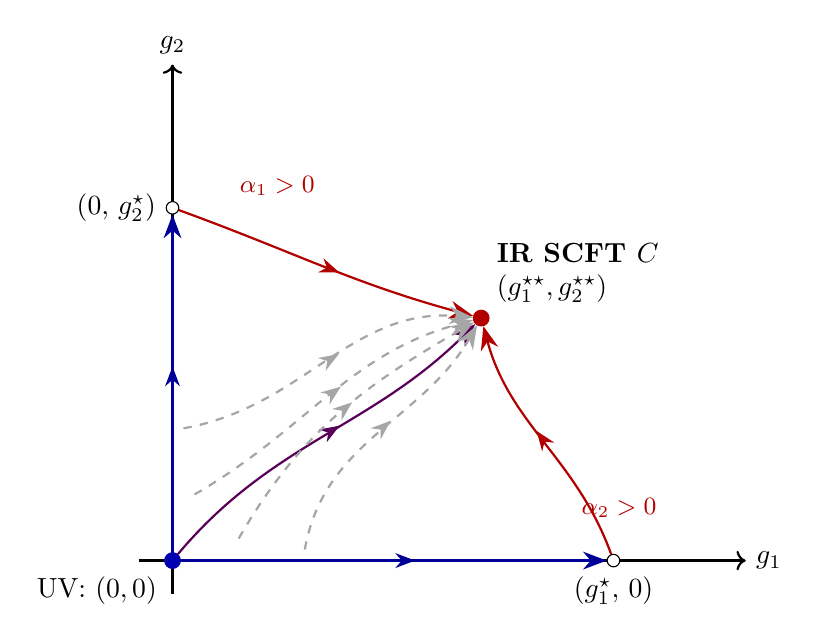
\begin{tikzpicture}[
    scale=1.4,
    flow/.style={thick, -{Stealth[length=3mm]},
      postaction={decorate},
      decoration={markings, mark=at position 0.55 with
        {\arrow{Stealth[length=2.5mm]}}}},
    fp/.style={circle, draw=black, fill=white, inner sep=1.6pt},
    fpIR/.style={circle, draw=red!70!black, fill=red!70!black, inner sep=2pt},
    fpUV/.style={circle, draw=blue!70!black, fill=blue!70!black, inner sep=2pt},
  ]
    % axes
    \draw[->, thick] (-0.3,0) -- (5.2,0) node[right] {$g_{1}$};
    \draw[->, thick] (0,-0.3) -- (0,4.5) node[above] {$g_{2}$};
    % fixed points
    \node[fpUV, label={below left:UV: $(0,0)$}] (UV) at (0,0) {};
    \node[fp,   label={left:$(0,\,g_{2}^{\star})$}]      (A1) at (0,3.2) {};
    \node[fp,   label={below:$(g_{1}^{\star},\,0)$}]     (A0) at (4.0,0) {};
    \node[fpIR, label={[align=left]above right:{\textbf{IR SCFT $C$}\\$(g_{1}^{\star\star},g_{2}^{\star\star})$}}]
          (IR) at (2.8,2.2) {};
    % flows from UV
    \draw[flow, blue!60!black] (UV) -- (A1);
    \draw[flow, blue!60!black] (UV) -- (A0);
    % off-axis flows away from boundary SCFTs
    \draw[flow, red!70!black] (A1) to[out=-20, in=165] (IR);
    \draw[flow, red!70!black] (A0) to[out=110, in=-75] (IR);
    % interior flow from UV
    \draw[flow, violet!70!black] (UV) to[out=50, in=225] (IR);
    % generic trajectories
    \draw[flow, gray!70, dashed] (0.6,0.2) to[out=60, in=210] (IR);
    \draw[flow, gray!70, dashed] (0.2,0.6) to[out=30, in=195] (IR);
    \draw[flow, gray!70, dashed] (1.2,0.1) to[out=80, in=240] (IR);
    \draw[flow, gray!70, dashed] (0.1,1.2) to[out=10, in=175] (IR);
    % labels
    \node[red!70!black]  at (0.95, 3.40) {\small $\alpha_{1}>0$};
    \node[red!70!black]  at (4.05, 0.48) {\small $\alpha_{2}>0$};
  \end{tikzpicture}
  \caption{Figure~5 topology: $(\alpha_{1},\alpha_{2})=(+,+)$, both
    axis SCFTs are IR-unstable and release the flow into the
    interior; the two-coupling SCFT $C$ at
    $(g_{1}^{\star\star},g_{2}^{\star\star})$ is the global IR
    attractor.  Realised by class~$2$ in the $\SU(N)\times\SU(N)$
    non-Veneziano landscape.}
  \label{fig:fig5}
\end{figure}


% Inline TikZ: Figure 6 topology (both axes IR-stable, separatrix through saddle C)
\begin{figure}[h]
  \centering
  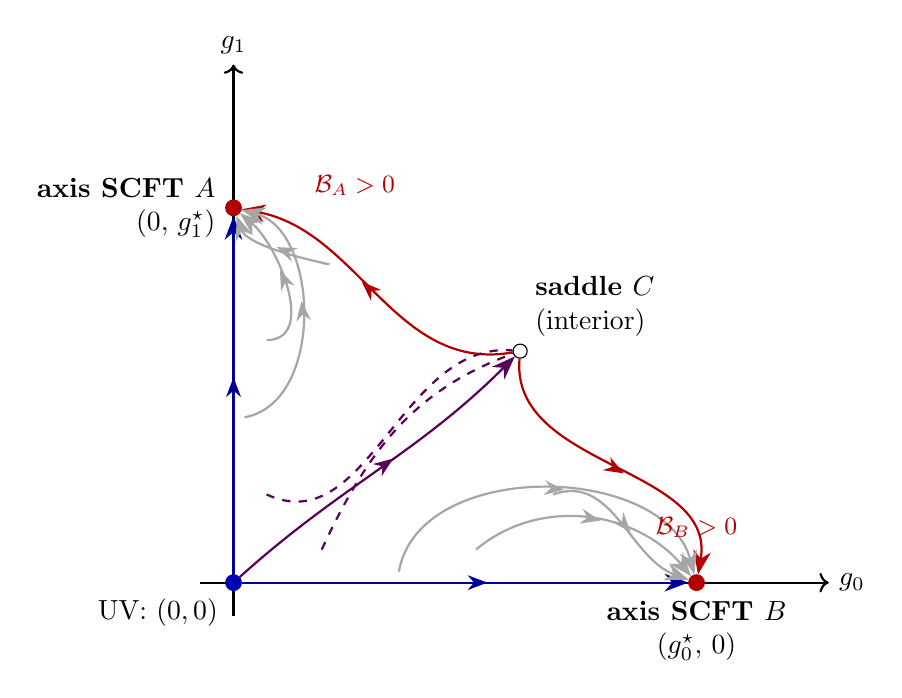
\begin{tikzpicture}[
    scale=1.4,
    flow/.style={thick, -{Stealth[length=3mm]},
      postaction={decorate},
      decoration={markings, mark=at position 0.55 with
        {\arrow{Stealth[length=2.5mm]}}}},
    fp/.style={circle, draw=black, fill=white, inner sep=1.8pt},
    fpIR/.style={circle, draw=red!70!black, fill=red!70!black, inner sep=2pt},
    fpUV/.style={circle, draw=blue!70!black, fill=blue!70!black, inner sep=2pt},
  ]
    % axes
    \draw[->, thick] (-0.3,0) -- (5.4,0) node[right] {$g_{0}$};
    \draw[->, thick] (0,-0.3) -- (0,4.7) node[above] {$g_{1}$};
    % fixed points
    \node[fpUV, label={below left:UV: $(0,0)$}] (UV) at (0,0) {};
    \node[fpIR, label={[align=right]left:{\textbf{axis SCFT $A$}\\$(0,\,g_{1}^{\star})$}}]
          (A1) at (0,3.4) {};
    \node[fpIR, label={[align=center]below:{\textbf{axis SCFT $B$}\\$(g_{0}^{\star},\,0)$}}]
          (A0) at (4.2,0) {};
    \node[fp,   label={[align=left]above right:{\textbf{saddle $C$}\\(interior)}}]
          (C)  at (2.6,2.1) {};
    % flows from UV up the two axes
    \draw[flow, blue!60!black] (UV) -- (A1);
    \draw[flow, blue!60!black] (UV) -- (A0);
    % axis fixed points ATTRACT off-axis flows
    \draw[flow, red!70!black] (C) to[out=190, in=-10] (A1);
    \draw[flow, red!70!black] (C) to[out=-95, in=80] (A0);
    % incoming trajectories to C along stable manifold (separatrix)
    \draw[flow, violet!70!black, thick] (UV) to[out=42, in=225] (C);
    % separatrix (continues past C on the unstable direction)
    \draw[dashed, thick, violet!70!black]
      (0.3,0.8) to[out=-25, in=175] (C);
    \draw[dashed, thick, violet!70!black]
      (0.8,0.3) to[out=65, in=200] (C);
    % basin A trajectories (end on A1)
    \draw[flow, gray!70] (0.1,1.5) to[out=10, in=-15] (A1);
    \draw[flow, gray!70] (0.3,2.2) to[out=0, in=-40] (A1);
    \draw[flow, gray!70] (0.8,2.9) to[out=-10, in=-70] (A1);
    % basin B trajectories (end on A0)
    \draw[flow, gray!70] (1.5,0.1) to[out=80, in=105] (A0);
    \draw[flow, gray!70] (2.2,0.3) to[out=40, in=130] (A0);
    \draw[flow, gray!70] (2.9,0.8) to[out=20, in=160] (A0);
    % B label
    \node[red!70!black]  at (1.1, 3.60) {\small $\Bcond_{A}>0$};
    \node[red!70!black]  at (4.20, 0.50) {\small $\Bcond_{B}>0$};
  \end{tikzpicture}
  \caption{Topology (iii): $\Bcond_{A},\Bcond_{B}>0$.  Both boundary
    single-node SCFTs (filled red circles) are IR-stable; a separatrix
    (dashed violet) through the interior saddle $C$ divides the basins
    of attraction.  Realised by class~$16$ deformed by $\Nf$
    fundamentals on node~$1$ in the window
    $0.427\,N-1<\Nf<N-1$.}
  \label{fig:fig6}
\end{figure}


\subsection{Deforming class~$16$ by fundamentals on node~$1$}
\label{sec:phases-class16}

We now deform the representative theory of class~$16$ by adding
$\Nf$ pairs of (anti-)fundamentals $(\fund+\afund)^{\Nf}$ to node~$1$
only, keeping node~$0$'s matter unchanged.  The effect on the two
boundaries is asymmetric because $\Nf$ enters the decoupled-sub-theory
a-maximisation only when node~$1$ is the \emph{active} node:

\begin{itemize}\setlength{\itemsep}{4pt}
  \item \textbf{Boundary A ($g_{1}=0$, node~$0$ active).}  The
    boundary sub-theory consists of node~$0$'s own $A+2\bar A$ tensors
    and the three bifundamentals promoted to fundamentals of
    $\SU(N)_{0}$.  The N\_f fundamentals on node~$1$ are free spectators
    and do not participate in the boundary-A a-max.  The a-maximal
    bifundamental R-charge at boundary A is independent of $\Nf$:
    \begin{equation}
      R_{\text{bif}}^{(A)}\;=\;\tfrac{1+\sqrt{5}}{6}\;\simeq\;0.539\,.
    \end{equation}
    The corrected AF bound on the free node~$1$ is therefore
    \begin{equation}
      \Nf\;\le\;\alpha^{(A)}_{\Bcond}\,N
      +2\gamma^{(A)}_{\Bcond}\;=\;0.427\,N-1\,,
      \label{eq:class16-BcondA}
    \end{equation}
    where the coefficient $\alpha^{(A)}_{\Bcond}=3\cdot\tfrac{1}{2}
    \cdot 1\cdot(3R_{\text{bif}}^{(A)}-2)+\alpha^{(1)}_{0}$ with
    $\alpha^{(1)}_{0}=1$.  Thus
    \begin{equation}
      \Bcond_{A}<0\;\Longleftrightarrow\;\Nf<0.427\,N-1\,,
    \end{equation}
    i.e.\ exceeding the corrected AF bound flips boundary~A from
    IR-unstable to IR-stable.

  \item \textbf{Boundary B ($g_{0}=0$, node~$1$ active).}
    Node~$1$'s matter now includes its own $\bar A$ tensor, three
    bifundamentals (as flavours), \emph{and} the $\Nf$ fundamentals.
    The a-maximisation for this sub-theory changes as $\Nf$ is varied.
    At $\Nf=0$ the stored database value is
    $\alpha^{(B)}_{\Bcond}\,N+2\gamma^{(B)}_{\Bcond}=-0.573\,N+1$,
    corresponding to $\Bcond_{B}>0$ (axis~B IR-stable) at all $N\ge 2$.
    Adding $\Nf>0$ increases $R_{\text{bif}}^{(B)}$ towards the
    free-field value $2/3$, reducing $|3R_{\text{bif}}^{(B)}-2|$ and
    driving $\alpha^{(B)}_{\Bcond}$ towards $0$ from below;
    it does not change sign within the AF window $\Nf<N-1$.
\end{itemize}

The UV asymptotic-freedom of node~$1$ requires $\Nf<N-1$; node~$0$'s
AF is unchanged because none of its matter is altered.  Combining
these with the boundary analyses above yields the phase diagram
summarised in Table~\ref{tab:class16-phases}.

\begin{table}[h]
  \centering
  \begin{tabular}{lcccc}
    \toprule
    Window on $\Nf$ (node~$1$) & $b_{0}^{(0)}$ & $b_{0}^{(1)}$
                               & $\Bcond_{A}$  & $\Bcond_{B}$
                               \\
    \midrule
    $0\le \Nf<0.427\,N-1$ &$+$&$+$&$<0$&$>0$\\
    $0.427\,N-1<\Nf<N-1$ &$+$&$+$&$>0$&$>0$\\
    $\Nf\ge N-1$          &$+$&$\le 0$ &\multicolumn{2}{c}{--- not AF ---}\\
    \bottomrule
  \end{tabular}
  \caption{RG phase structure of class~$16$ as a function of the
    number of fundamental pairs $\Nf$ added to node~$1$.  The second
    row is the Figure~6 window.}
  \label{tab:class16-phases}
\end{table}

\subsection{Main result: explicit realisation of
  \texorpdfstring{\cite[Fig.~6]{IW2005}}{Intriligator--Wecht Figure 6}}
\label{sec:phases-main}

Combining the two boundary analyses with the UV-AF budget, we
conclude:

\begin{quote}
  \textbf{Theorem (main result).}  The $\SU(N)\times\SU(N)$
  quiver gauge theory with:
  \begin{itemize}\setlength{\itemsep}{1pt}
    \item node-$0$ matter $A+2\bar A$;
    \item node-$1$ matter $\bar A$ plus $\Nf$ vector-like pairs
      $(\fund+\afund)^{\Nf}$;
    \item three bifundamentals of structure
      $2\,(\fund_{0},\fund_{1})+(\afund_{0},\afund_{1})$;
  \end{itemize}
  is UV-asymptotically free and realises the two-boundary
  IR-stable RG topology of \cite[Fig.~6]{IW2005} in the window
  \begin{equation}
    0.427\,N-1\;<\;\Nf\;<\;N-1.
    \label{eq:main-theorem-window}
  \end{equation}
  For $N\ge 4$ this window is non-empty, and its width grows
  linearly with $N$ as $\approx 0.573\,N$.  In this window the
  two boundary fixed points attract generic flows; the interior
  R-symmetry extremum $C$ is not an attractor.
\end{quote}

This is the first explicit realisation, to our knowledge, of
\cite[Fig.~6]{IW2005}, answering the remark of those authors that
such examples had not been found.

\subsection{Remarks on the interior fixed point in the Figure~6 phase}
\label{sec:phases-interior}

The interior extremum $C$ exists algebraically throughout the window:
the symbolic $a$-maximisation of the deformed class~$16$ returns a
non-degenerate critical point in the R-charge polytope at every
$\Nf$ in \eqref{eq:main-theorem-window}.  However, the sign pattern
$(\Bcond_{A},\Bcond_{B})=(+,+)$ at both boundaries forces $C$ to be a
saddle of the two-coupling flow, \emph{not} a local attractor, and
hence $C$ does not describe the IR of generic trajectories in the
interior.  The two axis SCFTs --- the $\SU(N)_{0}$ single-node SCFT on
the $g_{0}$-axis and the $\SU(N)_{1}$ single-node SCFT on the
$g_{1}$-axis --- are both IR-stable attractors with finite basins
separated by the (co-dim $1$) stable manifold of $C$.

We emphasise that the Figure~6 phase is accessible within the
classified database by a \emph{single-parameter} deformation: only
$\Nf$ on node~$1$ is varied, and only one of the five interacting
classes (class~$16$) realises it.  The remaining four classes
($4$, $21$, $23$) in the mixed topology do not enter the Figure~6
window under analogous deformations, because either $\alpha^{(A)}_{\Bcond}$
or $\alpha^{(B)}_{\Bcond}$ has the wrong sign from the outset for the
corresponding deformation.

A fully quantitative characterisation of the separatrix basin
structure (position of $C$ in the $(g_{0},g_{1})$ plane, slope of the
separatrix near $C$, and basin area ratios) requires going beyond the
one-loop analysis employed here; this is left for future work.


% ══════════════════════════════════════════════════════════════════════
\section{Discussion}
\label{sec:discussion}

% ══════════════════════════════════════════════════════════════════════
% § 6  Discussion
% ══════════════════════════════════════════════════════════════════════

\subsection{Summary}

We have classified all four-dimensional $\N=1$ asymptotically free
$\SU(N)\times\SU(N)$ quiver gauge theories in the equal-rank,
non-Veneziano large-$N$ sector, using symbolic $a$-maximisation to
compute IR R-charges and central charges.  Nine universality classes
emerge; every class with a defined leading-$N$ $a$-maximum satisfies
$a=c$ to leading order in $1/N$.

Applying the boundary analysis of \cite{IW2005}, we have computed the
boundary one-loop coefficients $b_{0}^{(a)}(g_{b}^{\star})$ for every
class and classified each by the sign pattern
$(\text{sign}\,\alpha_{1},\text{sign}\,\alpha_{2})$ of the
leading-$N$ coefficients.  Class 2 realises the Figure~5 topology;
classes $4,16,21,23$ realise a mixed topology in which one axis SCFT
attracts generic flows; class 44 is leading-$N$ marginal at both
boundaries.  Classes $1$, $9$, and $877$ together with the 20
flat-direction theories excluded from the nine-class tabulation form
a single \emph{nonSCFT} umbrella: in each case the leading-$N$
$a$-maximisation does not identify a unitary interacting SCFT, either
because it returns R-charges below the unitarity bound (classes 1, 9,
877 — at $R=0$, $R=1/2$, and $R=0$ on surviving matter respectively)
or because the critical point is not a genuine local maximum (flat
direction).  Class 877 is further singled out by its empty-node
morphology: the 9 surviving representatives admit a unique interior
$a$-maximum at $a/N^{2}=0$, but the sub-quiver decoupling limit
required for the boundary analysis is subtle for an all-bifundamental
matter sector and is left for a separate treatment.

Our main result is that the strictly non-Veneziano landscape contains
no Figure~6 realisation, but that a simple single-parameter Veneziano
deformation of class~16 (adding $\Nf^{(2)}$ fundamental pairs to
node~2 in the window $0.427\,N-1<\Nf^{(2)}<N-1$) produces precisely
the both-axes-stable RG topology of \cite[Fig.~6]{IW2005}.  The
interior $a$-maximal critical point persists as a saddle inside this
window, and the two axis SCFTs become the IR attractors with basins
separated by the stable manifold of the saddle.  This is, to our
knowledge, the first explicit realisation of this RG topology.

\subsection{Implications}

\paragraph{$a=c$ in the equal-rank non-Veneziano sector.}  The
uniform appearance of $a=c$ across all classes with a defined
leading-$N$ central charge suggests the non-Veneziano restriction is
itself the relevant filter: the
subleading, flavour-asymmetric contribution to $\Tr R^{3}-\Tr R$ that
would distinguish $a$ from $c$ is generically the
$\mathcal O(N)$-many fundamentals' contribution, and setting
$\Nf=\mathcal O(N^{0})$ removes it at leading order.  Quantifying the
sub-leading $a-c$ split as a function of a Veneziano parameter
$x^{(a)}=\Nf^{(a)}/N$ is a natural extension.

\paragraph{Holographic dual of the Figure~6 phase.}  In the Figure~5
topology, the single interior SCFT that attracts generic flows
admits a holographic interpretation through a single interior AdS
throat.  The Figure~6 topology, by contrast, has two distinct IR
attractors on the axes; a holographic dual would require a bulk
geometry with two separate IR asymptotic regions, connected in the
UV, selected by the UV Wilsonian initial condition.  Whether the
deformed class~16 realises such a bulk dual --- and whether the
separatrix structure admits a gravity interpretation --- is an open
question.

\paragraph{Higher-loop robustness.}  The boundary criterion used here
is one-loop via NSVZ and linear in the bifundamental anomalous
dimension.  Two- and higher-loop corrections can shift the
sign-flip thresholds by $\mathcal{O}(1/N)$ amounts.  The lower edge
of the class-16 Figure~6 window at $\Nf^{(2)}=0.427\,N-1$ is
therefore expected to receive $\mathcal{O}(1/N)$ corrections; the
upper edge $\Nf^{(2)}=N-1$ is the UV-AF cliff and is exact.  Because
the boundary coefficient $\alpha_{2}=-0.5730$ on axis 2 is
$\mathcal{O}(N)$ and of definite sign throughout the window, the
qualitative Figure~6 phase assignment is robust against higher-loop
corrections.

\paragraph{Boundary-versus-interior $R_{\text{bif}}$.}  We have used
the interior $R_{\text{bif}}$ (from full-theory $a$-maximisation) as
a leading-$N$ proxy for the boundary sub-theory $R_{\text{bif}}$.
The two prescriptions agree qualitatively (same sign pattern) under
the mild assumption that neither has $R_{\text{bif}}$ cross the
free-field value $2/3$, which holds for all classes with a defined
interior $a$-maximum.  A
refinement using the strict sub-theory $a$-max for the boundary
R-charges would change the quantitative value $0.427$ at the
Figure~6 lower edge by $\mathcal O(1/N)$ but not alter the existence
or the width-scaling $\approx 0.573\,N$ of the window.

\subsection{Future work}
\label{sec:future}

\begin{itemize}
  \item \textbf{$n$-node quivers.}  Extending this analysis to linear
    and cyclic quivers with $n\ge 3$ nodes requires a
    $2^{n}$-dimensional sign-pattern analysis on the boundaries; we
    expect richer topologies including partial basins and sub-quiver
    attractors.
  \item \textbf{$\SO/\Sp$ sectors.}  The database also contains
    $\SU$--$\SO$, $\SU$--$\Sp$ and $\SO$--$\Sp$ two-node theories.  A
    parallel analysis of these mixed-group sectors in the
    non-Veneziano limit should uncover additional realisations of the
    three topologies and possibly new Figure~6 windows.
  \item \textbf{Sub-leading treatment of class~44 and of the nonSCFT
    umbrella.}
    Class 44's boundary coefficients vanish at leading $N$; the
    subleading structure would determine its RG topology exactly.
    The nonSCFT umbrella — classes 1, 9, 877 and the 20
    flat-direction theories — is where the leading-$N$ $a$-maximisation
    fails to identify a unitary interacting SCFT: classes~1 and~9
    have R-charges below unitarity ($R=0$ and $R=1/2$), class~877 has
    $a/N^{2}=0$ with all surviving matter R-charges vanishing and
    additionally requires a separate sub-quiver decoupling treatment
    because its empty-node morphology places all matter on
    bifundamentals, and the flat-direction theories have
    non-uniquely-determined IR R-charges.  Lifting any of these into
    the interior of the polytope by sub-leading corrections (or
    finding a different R-symmetry extremum) would give their
    physical IR.
  \item \textbf{Other mixed-phase Figure~6 candidates.}  Class 21
    admits a narrow window $0.6754\,N+2<\Nf^{(1)}<N+2$ that may
    give a second Figure~6 realisation under analogous deformation;
    because class 21's node 2 is leading-$N$ marginal, a careful
    sub-leading analysis is needed to confirm this.
  \item \textbf{Explicit two-coupling RG numerics.}  Numerical
    integration of the two-coupling NSVZ flow in the
    $(g_{1},g_{2})$-plane, with R-charges updated self-consistently
    along the trajectory, would make the separatrix and basin
    structure in the class-16 Figure~6 window fully manifest.
  \item \textbf{Veneziano phase diagram.}  The sign-flip
    $\alpha_{1}<0\to\alpha_{1}>0$ at $\Nf^{(2)}=0.427\,N-1$ is the
    boundary of the Figure~6 phase in the $(\Nf^{(1)},\Nf^{(2)})$
    plane for class~16.  Mapping out the full two-dimensional phase
    diagram in $(x^{(1)},x^{(2)})$ Veneziano parameters would
    generalise the present results to the Veneziano regime and
    naturally connect to the full database.
\end{itemize}

\paragraph{Acknowledgements.}  We thank the organisers of [...] for
useful discussions.  Computations were performed with the symbolic
$a$-maximisation pipeline described in the companion code repository.


% ══════════════════════════════════════════════════════════════════════
\appendix
\section{Mixed-rank $\SU(m_{0}N)\times\SU(m_{1}N)$ classes}
\label{app:mixed}

% ══════════════════════════════════════════════════════════════════════
% Appendix A  Mixed-rank SU-SU no-Veneziano classes
% ══════════════════════════════════════════════════════════════════════

In the main text we focused on the equal-rank case
$\SU(N)_{0}\times\SU(N)_{1}$ with rank multipliers $(m_{0},m_{1})=(1,1)$.
The same classification pipeline may be run at general coprime rank
multipliers, producing additional non-Veneziano universality classes
for
\begin{equation}
  G\;=\;\SU(m_{0}N)_{0}\times\SU(m_{1}N)_{1},
  \qquad\gcd(m_{0},m_{1})=1\,,
\end{equation}
with $(m_{0},m_{1})$ chosen up to a swap of the two nodes.  We retain
only classes with $m_{0},m_{1}\le 4$.

\paragraph{Inventory.}  Table~\ref{tab:mixed-rank-inventory} lists the
$20$ mixed-rank non-Veneziano classes with $a_{/N^{2}}$ defined.
As in the equal-rank case, every non-degenerate class saturates
$a=c$ to leading order in $1/N$.

\begin{table}[h]
  \centering
  \small
  \begin{tabular}{cccrll}
    \toprule
    Class & $m_{0}$ & $m_{1}$ & \# theories & $a/N^{2}$ & $a/c$ \\
    \midrule
    $111$ & $2$ & $1$ & $2$  & $-0.6328$ & $1.0$ \\
    $117$ & $2$ & $1$ & $2$  & $0$ & (deg.) \\
    $121$ & $2$ & $1$ & $8$  & $0.7910$ & $1.0$ \\
    $122$ & $2$ & $1$ & $8$  & $0.7922$ & $1.0$ \\
    $134$ & $2$ & $1$ & $8$  & $1.0547$ & $1.0$ \\
    $136$ & $2$ & $1$ & $16$ & $1.0760$ & $1.0$ \\
    $153$ & $2$ & $1$ & $20$ & $1.1470$ & $1.0$ \\
    $159$ & $2$ & $1$ & $3$  & $1.1897$ & $1.0$ \\
    $160$ & $2$ & $1$ & $40$ & $1.1926$ & $1.0$ \\
    $174$ & $2$ & $1$ & $6$  & $1.25$ & $1.0$ \\
    $283$ & $3$ & $1$ & $8$  & $0.9722$ & $1.0$ \\
    $298$ & $3$ & $1$ & $20$ & $2.3056$ & $1.0$ \\
    $377$ & $3$ & $2$ & $8$  & $2.2222$ & $1.0$ \\
    $384$ & $3$ & $2$ & $34$ & $2.4668$ & $1.0$ \\
    $398$ & $3$ & $2$ & $20$ & $2.5477$ & $1.0$ \\
    $437$ & $3$ & $2$ & $12$ & $2.9722$ & $1.0$ \\
    $450$ & $3$ & $2$ & $88$ & $3.1192$ & $1.0$ \\
    $681$ & $4$ & $3$ & $34$ & $4.9951$ & $1.0$ \\
    $730$ & $4$ & $3$ & $12$ & $5.9425$ & $1.0$ \\
    $731$ & $4$ & $3$ & $88$ & $5.9568$ & $1.0$ \\
    \bottomrule
  \end{tabular}
  \caption{Mixed-rank non-Veneziano $\SU(m_{0}N)\times\SU(m_{1}N)$
    universality classes with $m_{0}\ne m_{1}$ (or $m_{0}=m_{1}>1$).
    $a/N^{2}$ is quoted to four decimal places; exact forms are
    available in the accompanying database.}
  \label{tab:mixed-rank-inventory}
\end{table}

\paragraph{RG phase distribution.}  Running the boundary analysis of
Section~\ref{sec:boundary} on each mixed-rank class reveals the same
three topology types (i), (ii), (iii) as in the equal-rank sector.
As in Section~\ref{sec:boundary-phases}, \emph{none} of the
non-Veneziano mixed-rank classes realise topology (iii) at $\Nf=0$.
Single-parameter deformations analogous to the class-$16$ deformation
of Section~\ref{sec:phases-class16} can push individual classes into
the Figure~6 window; characterising which mixed-rank classes admit a
Figure~6 phase is a straightforward but tedious exercise we leave for
future work.

\paragraph{Negative $a/N^{2}$.}  Class $111$ has a negative value of
the $a$-maximum at leading order, which violates the expected
positivity of $a$ for a unitary SCFT.  The negative value signals
that the $a$-max critical point at this order is not within the
physical R-symmetry polytope, and the theory is either non-unitary or
its leading-$N$ analysis misses a relevant sub-leading correction.
We flag this class as a cautionary boundary case rather than including
it in the topology-classification tables.


% ══════════════════════════════════════════════════════════════════════
\bibliographystyle{unsrt}
\bibliography{references}

\end{document}
